\documentclass[twocolumn, 11pt]{article}


\usepackage{csquotes}
\usepackage{amsmath}
\usepackage[utf8]{inputenc}
\usepackage[T1]{fontenc}
\usepackage[usenames]{color}
\usepackage{graphicx}
\usepackage[scaled=0.8]{luximono}
\usepackage{listings}
\usepackage{wrapfig}
\usepackage{multicol}
\usepackage{wasysym}

\graphicspath{{figures/}}

% ----- listings

\lstdefinelanguage{Scala}%
{morekeywords={abstract,%
  case,catch,char,class,%
  def,else,extends,final,finally,for,%
  if,import,implicit,%
  match,module,%
  new,null,%
  object,override,%
  package,private,protected,public,%
  for,public,return,super,%
  this,throw,trait,try,type,%
  val,var,%
  with,while,%
  yield%
  },%
  sensitive,%
  morecomment=[l]//,%
  morecomment=[s]{/*}{*/},%
  morestring=[b]",%
  morestring=[b]',%
  showstringspaces=false%
}[keywords,comments,strings]%

\lstset{language=Scala,%
  mathescape=true,%
%  columns=[c]fixed,%
%  basewidth={0.5em, 0.40em},%
  aboveskip=1pt,%\smallskipamount,
  belowskip=1pt,%\negsmallskipamount,
  lineskip=-0.2pt,
  basewidth={0.54em, 0.4em},%
%  backgroundcolor=\color{listingbg},
  basicstyle=\linespread{0.4}\footnotesize\ttfamily,
  keywordstyle=\keywordstyle,
%  commentstyle=\commentstyle
  xleftmargin=1ex
}

\definecolor{listingbg}{RGB}{240, 240, 240}

\newcommand{\commentstyle}[1]{\slseries{#1}}
\newcommand{\keywordstyle}[1]{\bfseries{#1}}

\lstnewenvironment{listing}{\lstset{language=Scala}}{}
\lstnewenvironment{listingtiny}{\lstset{language=Scala,basicstyle=\scriptsize\ttfamily}}{}

\newcommand{\code}[1]{\lstinline[language=Scala,columns=fixed,basicstyle=\ttfamily]|#1|}

\setlength{\parindent}{0pt}
\setlength{\parskip}{0.5\baselineskip plus 0.5\baselineskip minus 0.25\baselineskip}

\begin{document}

\newcommand{\lln}[1]{
  \lstinline@#1@
}

\title{Ruled Random Generation}
\author{Val\'erian Pittet}
\date{\today}

\onecolumn

\maketitle
\begin{abstract}

This project builds a programming interface to randomly generate music according to user-defined grammars.
To reach this aim, it provides
a model to abstract differents components of a melody
a small embedded domain specific language to describe grammars,
a (weak) generation algorithm,
the ability to trigger a special generation after specified event
and a midi interface based on javax.sound.midi to output the results.

The current report is divided in three parts.
The first one presents the model, how melodies are generated and the key point of implementation.
The second one shows an incremental process of using provided features to tune a good generation.
The last one gives a subjective review of the project and discusses what could be improved.


\end{abstract}
\newpage
\tableofcontents
  


\twocolumn

\section{Introduction}    
% birth of the project

% Introduction
% rythm abstraction
% circumventing back looking and heavy constraints


When designing this project, the first aim was to use a musical model that clearly separates the tonal aspect (heights of notes) and the rhythm.
Having this kind of separation makes it very simple to radically change a generated slow melody into a quick and energetic one.

The next step was to use an harmonic progression as the backbone of the melody. A ponctual constraint ensuring that somtimes, the melody follows some harmonic rules.
Given the aim of ruled random generation, the grammars, well-known tool to generate controlled sequences, were naturally chosen as basic representation.
However, the result : a set of parameters modeling a music generated using grammars, was not satisfying.

Indeed it lacks the ability to produce specific intended events. An event is characterized by two elements : the \emph{what} and the \emph{when}. The \emph{what} was relatively simple to explicit. It must be a way to restrict the generating grammars. The \emph{when} needed more research. The first attempt to specify the \emph{when} used a pattern recognition approach. ``If I see A generated then I trigger event E''. Unfortunately, pattern recognition is hard and heavy. There is a better solution. As every element is generated according to a grammar, at any point it is possible to know what pattern (of the grammar) has been and is being generated.

That is why the grammars of this project have been provided the ability to trigger grammar restricting events. In the following, you will see how the musical model is concretely build, the key points of the realization and how the code can be used to parametrize good generation.



\section{Technical aspect}
This section presents in detail the scheme of implementation and the key elements with theirs functionalities.


\subsection{Model}


This project proposes a ruled generation of music based on grammars, enhanced with events abilities.

The melodies are modeled through four different elements representing a sequence of musical cells (figure \ref{fig:concept}).
A cell is defined by one chord, one total duration (called root rythm), one rythmic pattern and a sequence of tones.
Each of those four components are generated from user-defined grammars. To avoid confusion between a character object of programmation and a character generated by a grammar, I call ``word'' the non-epsilon terminals generated by a grammar.

The chord grammar simply generates a sequence of chords, one per cell, ideally a harmonic progression.
The root rythm grammar gives the duration of the cell, hence one duration per cell is required.
The ryhmic pattern is represented with a sequence of rhythic cells. One word is one rhythmic cell. A rhythmic cell is a sequence of durations that compose a rhythm, for example figure \ref{fig:ncc}. Since the total duration of the rhythmic cell may not match the imposed duration of the cell, the rhythmic cell has to be strectched or shrinked. If the figure \ref{fig:ncc} is generated for a cell with root duration of \quarternote, it will be transformed in figure \ref{fig:cdcdc}

\onecolumn
\begin{figure}
  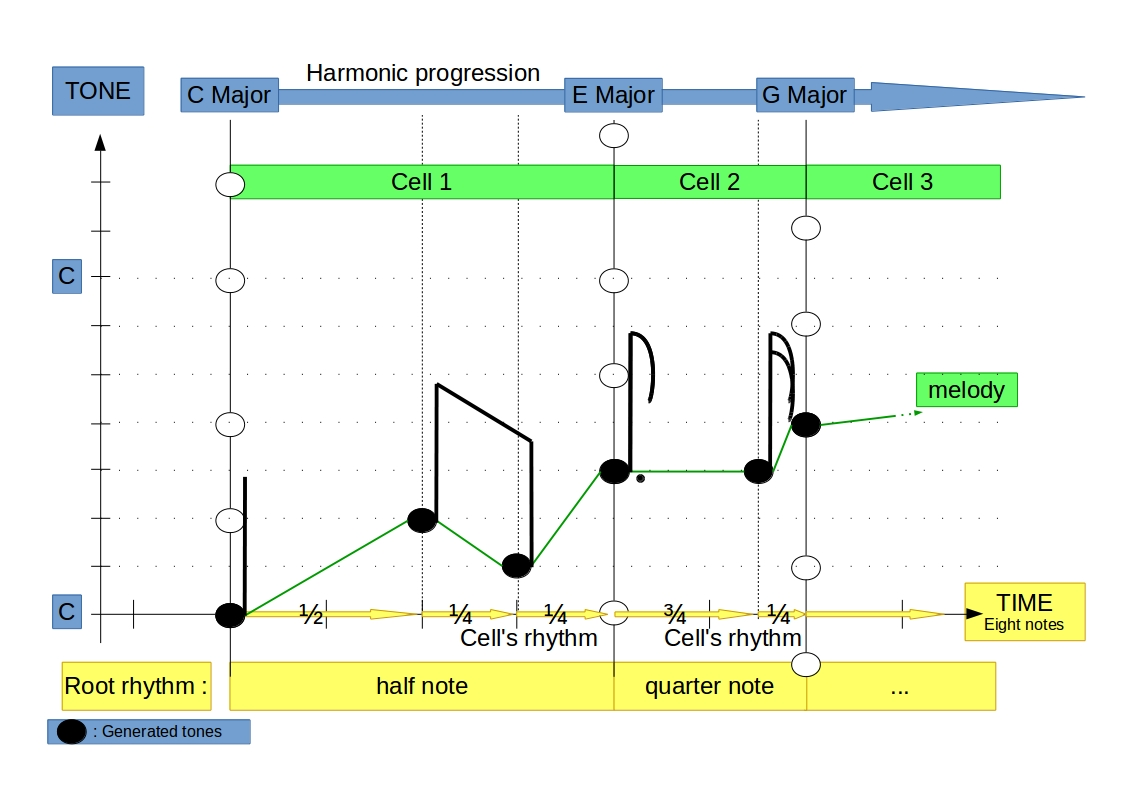
\includegraphics[width=\textwidth]{concept}
  \caption{Melody representation}
  \label{fig:concept}
\end{figure}
\twocolumn


\begin{figure}[h]
  \centering
  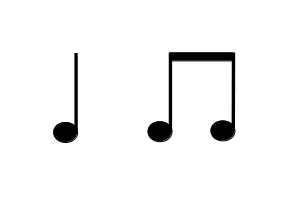
\includegraphics[scale=0.4]{ncc}
  \caption{Sample rhythmic cell}
  \label{fig:ncc}
\end{figure}

\begin{figure}[h]
  \centering
  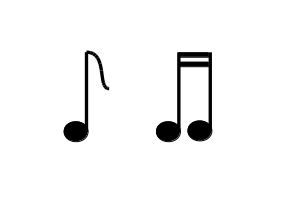
\includegraphics[scale=0.4]{cdcdc}
  \caption{Shrinked rhytmic cell}
  \label{fig:cdcdc}
\end{figure}

Finally the sequence of tones determines the height of the notes present in the cell. Unlike rhythmic cells, the melody grammar generates tone-by-tone words.
This choice represents the fact that rhythm is mostly repetitive and appears as small units while the melody is a flow of tones.
Obviously, the number of tones must match the size of the rhythmic cell (three in our small example).

At last, the first tone of a cell is required to be part of the chord of that cell. A note of any octave may be part of a chord, as long it has the 'right name'. The tone C at any octave is part of the C-Major chord.

To summarize, one cell :
\begin{itemize}
\item Starts with a tone of a provided chord
\item Lasts according to root rhythm
\item Contains a melody based on the rhythmic cell
\end{itemize}

With the four grammars, one cell is generated as follows :
\begin{itemize}
\item Chord grammar generates one more chord $c$
\item Root rhythm grammar generates one more word
\item Rhythmic cell grammar generates one more word of size $s$
\item Melody grammar generates $s$ tones such that the first one is in $c$
\end{itemize}

The sequence of cells is generated until some ending condition is reached, like the chord grammar reaches its end.
If the generation fails, for example the melody grammar did not allow to generate first tone of cell inside the chord, the longest successful sequence of cells is returned.
For more details about how multiple possibilities are managed and the specification of closing conditions please refer to section ``Generation Algorithm''.

\subsection{Grammar and Refinements}

As stated before, all generations are ruled by grammars. Because the aim is randomized generation with some control, alternatives must be provided with some weight that will indicate which choice to favor (figure \ref{fig:dummyGrammar}).
\begin{figure}[h]
  \centering
  \begin{lstlisting}
    A ::= 'c1' A       weight = 1.0
        | 'c2' 'c3' A  weight = 1.0
        | $\epsilon$             weight = 0.5
  \end{lstlisting}
  \caption{Weighted Grammar}
  \label{fig:dummyGrammar}
\end{figure}

The possibility of writing arbitrary grammars to generate the four melodic components already reaches a good flexibility. But this may not be enough. Indeed, there is very few control and communication possible between the differents components. The construction does not allow statements like ``if C-Major is generated, then the melody must be C-E-G''. But such concept is very useful to restrict and control generation.

That's why grammars are extended with the \emph{refinement} capability.
In a nutshell, a refinement is a message sent by a grammar A to a grammar B (A may equal B) that will restrict the generated sequence of B.

So, what implements a refinement ? Nothing else than another grammar. Note that the types of grammars must be equal. To refine the melody grammar, another melody grammar is required. Refining grammar A with A' consists in taking the conjuction of both grammars. This means that both must agree on generated words. What refinements do is a generalization of the following example.

Recall the two main purposes of a grammar: Parsing and generation. In parsing algorithms, a grammar is used to accept and derive abstract syntax tree of an input. The generation uses grammars to produce a sentence that matches the grammar.
In the current case, grammars are used as generators. But what happens if one wants to restrict the generated sentence ? He could put itself between parsing and generation and ask the grammar to parse a regular expression. The grammar rejects the regex if it is not feasible or returns the parsed regex with correct choices where words were not specified.

To get refinements, simply replace the regular expression by another grammar. The refinements are then simply inserted in the emitting grammar and behave like $\epsilon$ terminal that send messages to target grammar.

The transformation in grammar notation of the example mentionned above : ``if C-Major is generated, then the melody must be C-E-G'' is given in figure \ref{fig:refSam}. However, this refinement is very restricive and will likely fail unless initial melody grammar is flexible.

\begin{figure}[h]
  \centering
  \begin{lstlisting}
// chords grammar
Chords ::= .........
     /* replace all occurences of 'C-Major'
      * terminal by rule CM
      */ 

// new rule to send refinement
// before generating 'C-Major'
CM ::= RefineMelody(RM) 'C-Major'

// melody refinement
RM ::= 'C' 'E' 'G'

// melody grammar
Melody ::= .........

  \end{lstlisting}
  \caption{Refinement sample}
  \label{fig:refSam}
\end{figure}


Therefore this project uses grammars both as generator and parsor. That's why the term of Parsing Tree is used later, still Generation Tree may have been more accurate.

\subsection{Parsing Tree}


\code{ParsingTree} is the class of the program that stores an intermediate state of a grammar (figure \ref{fig:PT}). An intermediate state of a generative grammar represents which rules and terminals have been generated and what is left to generate. Intuitively, the generation is a path through the grammar's rules. The intermediate state describes which concrete path has been followed and what is planified to follow, which can contain non-deterministic choices to make.
To archieve this, \code{ParsingTree} stores two lists of grammar elements : The produced sentence and the stack of rules to apply. If the stack is empty, the generation is over.

\begin{figure}[h]
  \centering
  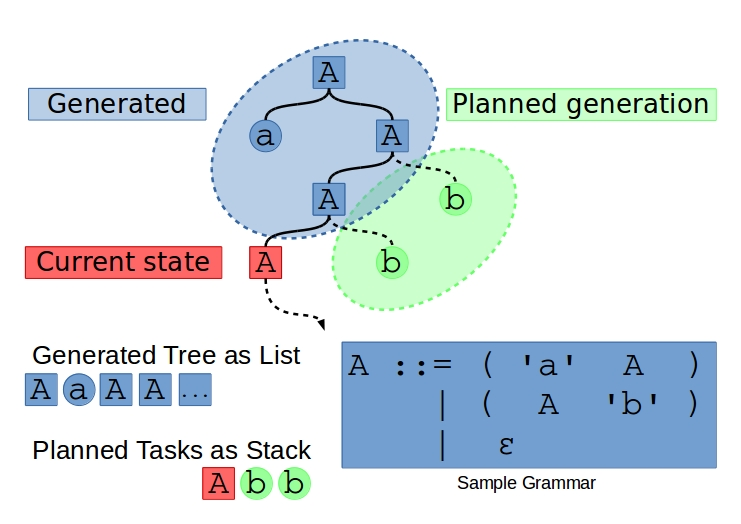
\includegraphics[width=0.5\textwidth]{parsingTree}
  \caption{Intermediate state}
  \label{fig:PT}
\end{figure}

\code{ParsingTree} also maintains a list of received refinements (also instances of \code{ParsingTree}) that restrict the generated sequence. The nexts possible words are defined by the intersection of the nexts words of the main grammar and all the refinements.

The main functionnality of \code{ParsingTree} is the function \code{nexts}. Upon \code{nexts} call, \code{ParsingTree} will generate a list of \emph{probable} \code{ParsingTree} that have generated one more word. The restriction of \emph{probable} is crucial. Recall that alternatives are weighted, they can thus be mapped to probabilities. Since the user-provided grammar may lead to unbounded possibilities (left-recursive grammars), computing the probability of each one is a good way to drop unprobable solutions and bound the result.


\subsection{Generation Algorithm}

As evoked in section ``Model'', this section presents how the generation algorithm manages multiple solutions and what are the possible ending solutions.

Taking everything into account, the generation problem is hard to express. There are four different grammars (Chords[C], Root rhythm[RR], Rhythmic cell[RC] and Melody[M]). For each \code{nexts} call, a \code{ParsingTree} may return multiple solutions and for a given cell the M grammar is not independant of C and RC. This means that They cannot be generated independantly and combined afterward.
The implemented generation algorithm is approximative and a good backtracking or equivalent approach would give better chances of success. However it is enough with few constraints when the theorical tree of all possible solutions has a large proportion of valid solutions.

There is how one cell is generated (figure \ref{fig:cellGen}). The four grammars are represented with \code{ParsingTree} to store intermediate state.
At the first step, there is the four-tuple \code{C, RR, RC, M}. The call \code{C.nexts} derives a first bunch of childrens. They are limited according to a fixed bound. The selection of childrens (unlike in the picture) is made randomly, according to probabilities derived from weights of the grammars rules. Then successively repeat this operation with \code{RR.nexts}, \code{RC.nexts} and \code{M.nexts}. When the new cells are generated \code{C', RR', RC', M'} if one fulfills the closing conditions (see next) then return that solution, otherwise generate another cell.

\onecolumn
\begin{figure}[d]
  \centering
  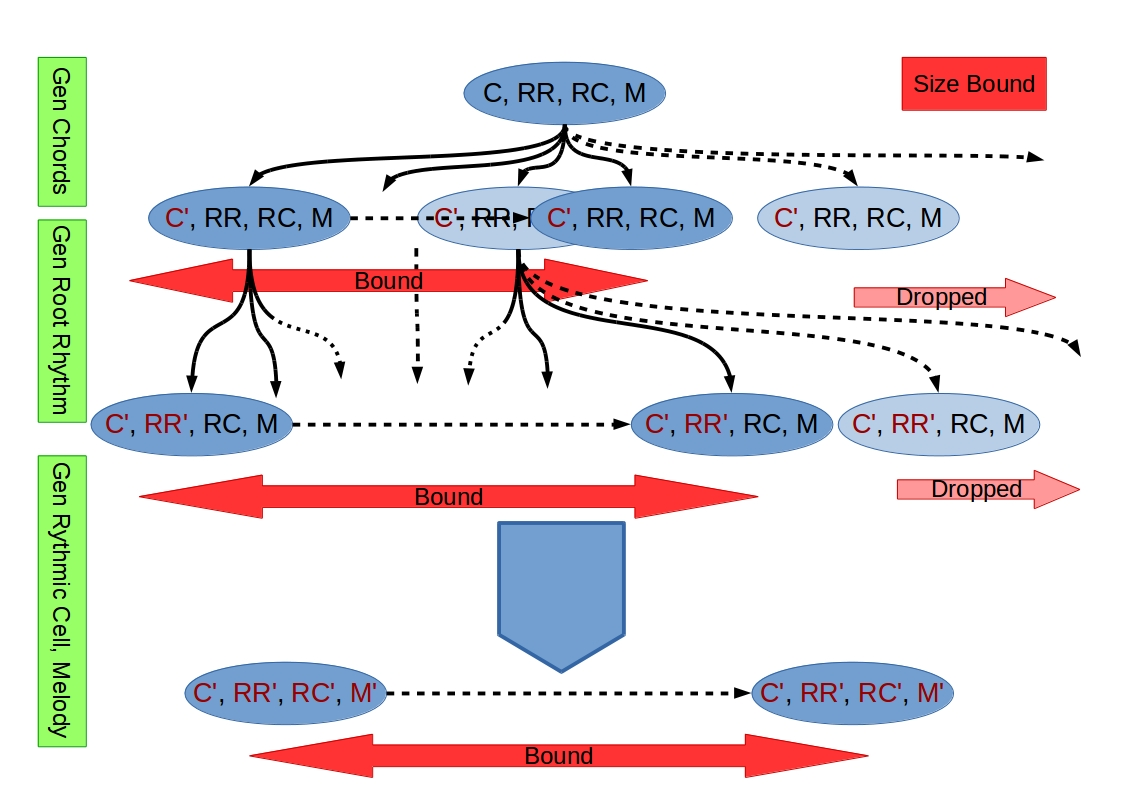
\includegraphics[width=\textwidth]{boundGen}
  \caption{Cell generation}
  \label{fig:cellGen}
\end{figure}
\twocolumn

% ending condition

Unlike the generation, the closing conditions are rather simple to formulate. The generation will always try to stop when the chord grammar reaches its end. This makes sence since the harmonic progression is the backbone of the melody. Then for each other grammar, the user can decide if they have to finish (the stack of planned generatio is empty) as well or not. This feature proves useful when one wants to precisely control the end of the generation (figure \ref{fig:endCTRL}).


\begin{figure}[h]
  \centering
  \begin{lstlisting}
// generative grammar
A ::= B A | E

// Body of grammar
B ::= ... /* some random generation */

// End of grammar
E ::= ... /* this must occur at end */
  \end{lstlisting}
  \caption{End Control}
  \label{fig:endCTRL}
\end{figure}


\section{Composition of an Example}

This section presents how to write grammars to generate a melody. At first, very simple grammars produce poor result, then incrementally using more features will enhance the generation to archieve an acceptable output.

To see source code and run samples according to different steps, feel free to clone the git repository of the project and checkout to the ``presentation'' branch.


\begin{lstlisting}
> git clone https://github.com/vtpittet/ScalaMusicGeneration
> cd ScalaMusicGeneration/MusicInterface/
> git checkout presentation
> sbt
> run
\end{lstlisting}


Then, you can select the class to run according to the name of the step you want to hear.
The source code is located in samples/Presentation.scala

For the sake of readability every grammar is written according to C-Major scale.
\subsection{Purely Random}

We first start with a simple deterministic chord sequence, the standard Tonic-Subdominant-Dominant-Tonic harmonic progression

\begin{lstlisting}
Chords ::= 'C-Major' 'F-Major' 'G-Major' 'C-Major'
\end{lstlisting}

Root rhythm and cell ryhthm are infinte sequences of one single element.

\begin{lstlisting}
Root ::= '$\halfnote$' Root
Cell ::= '$\quarternote \ \ \eighthnote  \eighthnote$'  Cell
\end{lstlisting}

Finally the tones, each step generating randomly one tone in the C-Scale in the base octave (figure \ref{fig:unif}).
All weights for alternatives are 1.0.

\begin{lstlisting}
Tones ::= ('C' | 'D' | 'E' | 'F' | 'G' | 'A' | 'B') Tones
\end{lstlisting}

\begin{figure}[h]
  \centering
  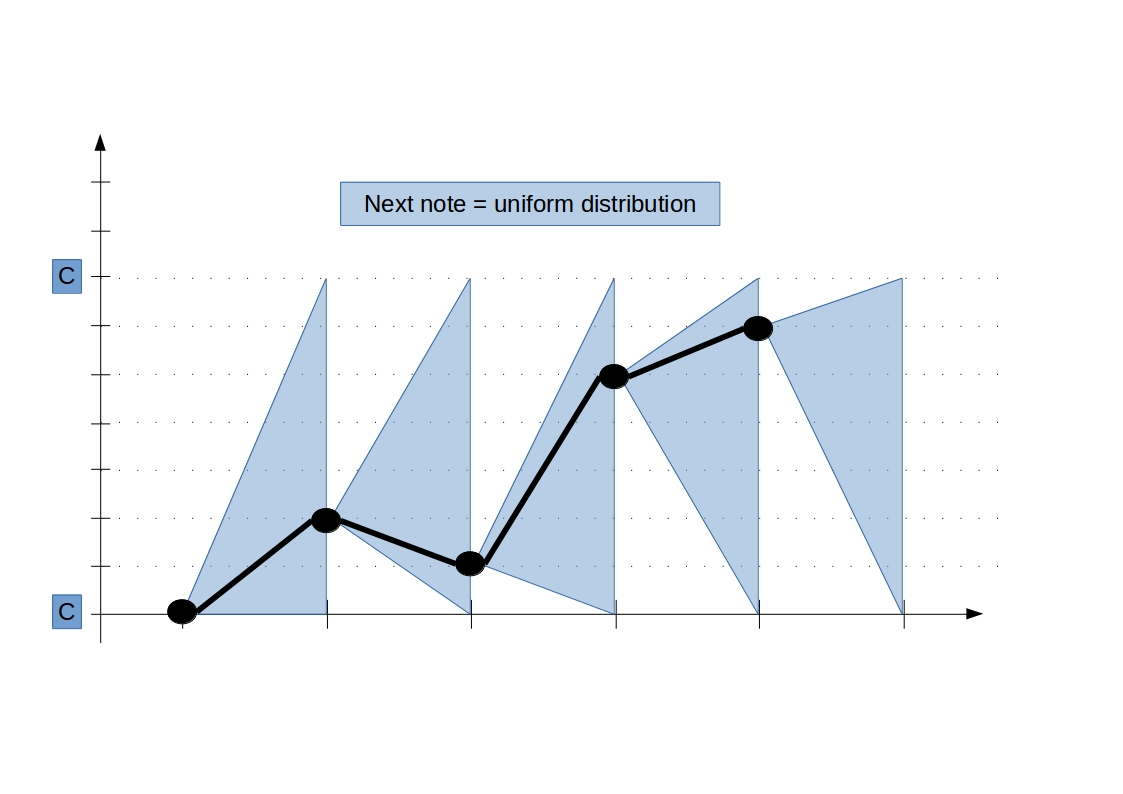
\includegraphics[width=0.5\textwidth]{uniform}
  \caption{Uniform Random Tones}
  \label{fig:unif}
\end{figure}
The generation follows default ending conditions. Only the chords sequence has to finish. Thus there is no trouble with the infinite grammars.

Generated melody is very poor. Let's see how to improve it.

\subsection{Flowing Melody}

Obviously the first fix is addressed to the tones generation.
The idea is to remember the previously generated tone to produce a close one to avoid big steps in the melody.

\begin{lstlisting}
C ::= 'C'
    (  B, w = 2.0
    |  C, w = 1.0
    |  D, w = 2.0)

D ::= 'D'
    (  C, w = 2.0
    |  D, w = 1.0
    |  E, w = 2.0)

// similar construction for E, F, G, A, B
E ::= ...
\end{lstlisting}

The C-rule produces a 'C' terminal and then can go to rule B, C or D, that behave similarly (figure \ref{fig:bound}).

\begin{figure}[h]
  \centering
  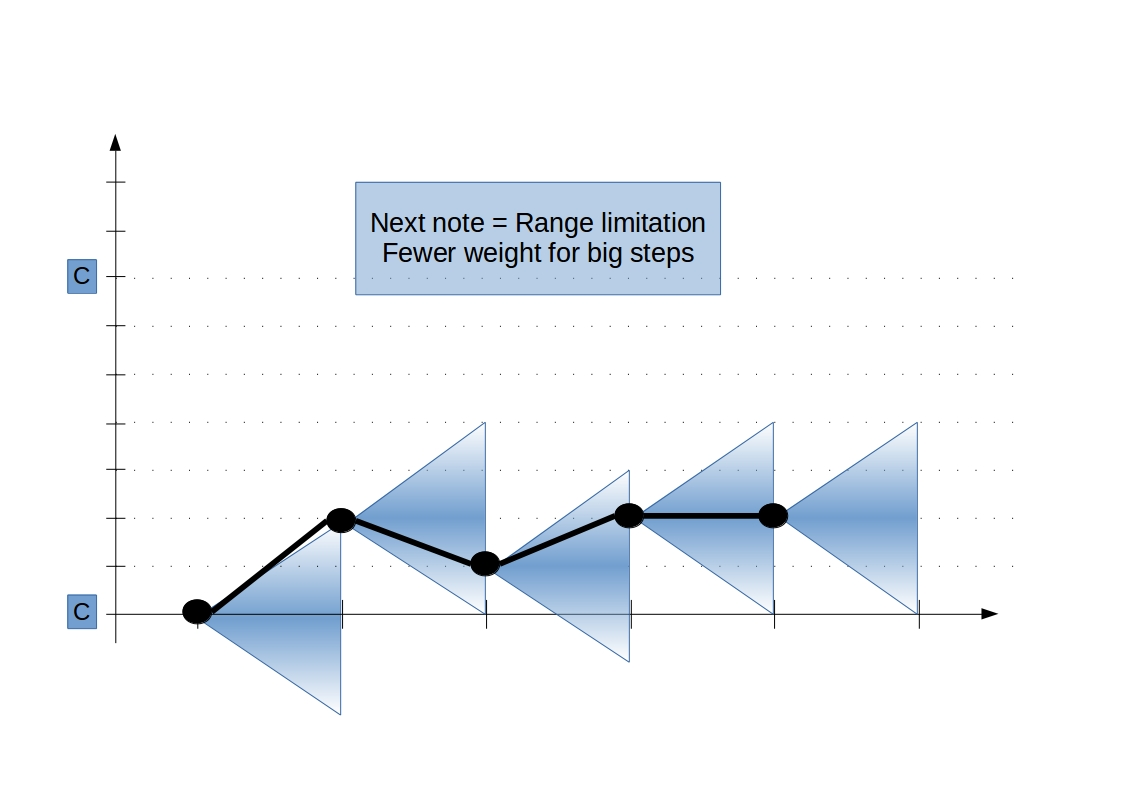
\includegraphics[width=0.5\textwidth]{bounded}
  \caption{Weights and Bounded Tones}
  \label{fig:bound}
\end{figure}


This is already much better.
In real Scala code, all rules ran be represented with a single \code{def} that takes the initial tone as parameter and returns the rule.
This functionnal approach allows to describe more complex grammar with only few lines that may have as additionnal parameter

Keeping the information of global movement of melody, the rules can adapt to follow global movement to generate a ``flowing'' melody (figure \ref{fig:inertial}).

\begin{figure}[h]
  \centering
  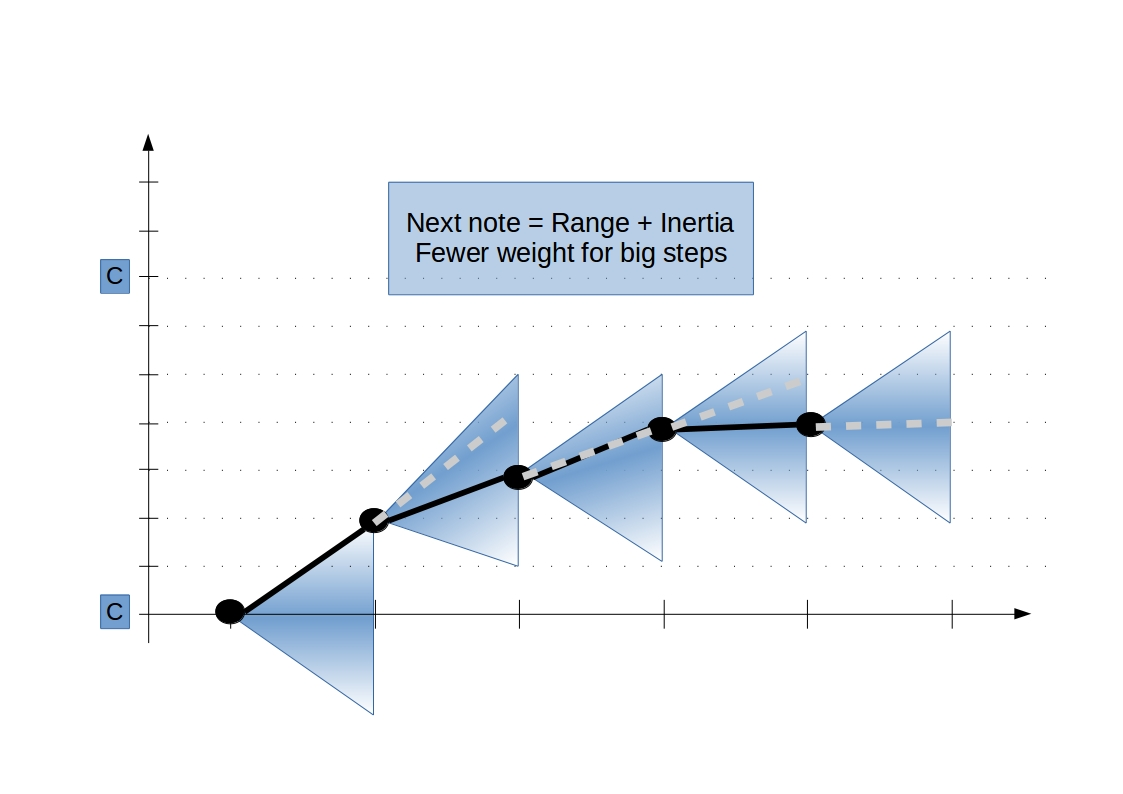
\includegraphics[width=0.5\textwidth]{inertial}
  \caption{Inertial Tone}
  \label{fig:inertial}
\end{figure}

\subsection{Harmony and Rhythm Variations}

Simply using more alternatives for chords and rhythms generation produces more diversity. All weights are set to one.
Chords has now three alternatives
\begin{lstlisting}
Chords ::= 'C-Major' B 'C-Major'

B ::= 'G-Major'
    | 'F-Major' 'G-Major'
    | 'F-Major' 'G-Major' 'G-Seventh'           
\end{lstlisting}


Each rhythmic component has two alternatives. This produce four different rhythm for the cells.
\begin{lstlisting}
Root ::= ('$\quarternote$' | '$\halfnote$') Root
Cell ::= ('$\quarternote \ \ \twonotes$' | '$\quarternote . \ \ \eighthnote$'  Cell
\end{lstlisting}

This simple way adds diversity and make the melody more interesting.

\subsection{End Specification}

In all the previous samples, the closing condition was on the chord sequence only. The produced melodies end abruptally and leave a feeling of incompleteness.
To solve this problem, the first point is to change the closing condition and require that every generated sequence must end simultaneously.
Then the grammars are adapted to be finite and there is only one way to finish the generation

The grammars must follow this pattern :


\begin{lstlisting}
A ::= (Body A, w = 1.0) | (End, w = 0.5)

Body ::= // list complex choices

End ::= // restricted end of generation
\end{lstlisting}

The bodies of grammars are unchanged and the ends are simply 'C' for Tones (we want to end on the tonic) and '\halfnote' for Root and Cells to close with a long single note.

Clearly the music ends much more neatly. However some runs still have a bad end. When the second to last note is very distant to the required last note (one octave lower for example) the end appears out of nowhere. The final enhancement fixes this problem using refinements.

\subsection{Refinements}

The proposition is to anticipate the end of the music and add a constraint to the Tones grammar that will make it converge towards the ending tone over the generation of $n$ tones.

This converging grammar is simply represented by a sequence of $n$ rules. The first one can generate $n$ different notes over and below C, the second one $n-1$, ... the nth one must generate the intended 'C' (figure \ref{fig:converge}).

\begin{figure}[h]
  \centering
  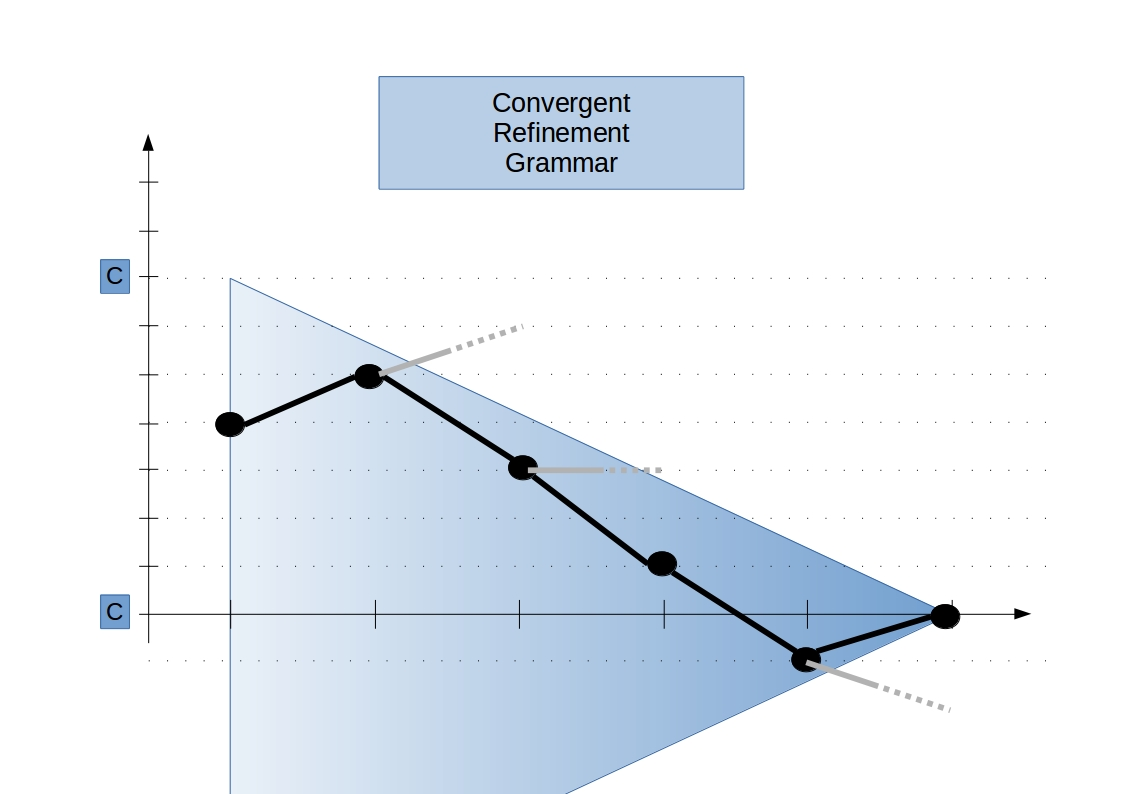
\includegraphics[width=0.5\textwidth]{converge}
  \caption{Convergent Refinement}
  \label{fig:converge}
\end{figure}

Finally the refinement is introduced inside the sequence of chords.

\begin{lstlisting}
// three times a harmonic sequence of chords
// then send refinement and produce last sequence of chords
FinalChords ::=
  Chords Chords Chords RefineMelody(RM) Chords

// converging grammar for melody
RM ::= ...
\end{lstlisting}


\section{Conclusion}

\subsection{Qualitative Evaluation}

\paragraph{Weakness of harmonic constraint}

It may appear that restricting only the first tone of a cell to match the provided chord is too weak. Indeed, it does not produce a complete harmonic progression on each note and the melody has a lot of freedom.

However, this constraint is not useless. People were asked to compare generations with and without this restriction and gave an interesting observation.
The melodies themselves were hard to compare, but in the latter case, the rhythm seemed degenerated. One interpretation is that the presence of the harmonic constraint at the beginning of the cells is passively perceived and produce an emphasis that evokes a reference point to interpret the music.

On the other hand it is still possible but more cumbersome to generate a melody where all notes match a harmonic progression. Use the root rhythm as the only rhythmic component and produce one infinite sequence of singleton rhythmic cell (figure \ref{fig:singleTonRC})

\begin{figure}[h]
  \centering
  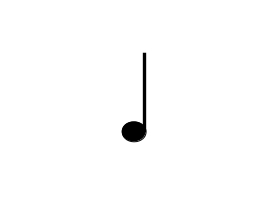
\includegraphics[scale=0.4]{n}
  \caption{Singleton Rhythmic Cell}
  \label{fig:singleTonRC}
\end{figure}



\paragraph{Generation algorithm}

The generation algorithm is simple and not very efficient. It cannot generate when the rules are too complex. Additionnaly, the usage of probabilities to limit the result, a good solution for simple cases, make it hard to predict the result. Suppose one wants to control the end of the melody and adds the tone grammar to ending conditions. If the ending path is long and its weight is small, it will never be kept long enough to reach the ending state. Thus when the chord grammar will reach its end, there will be no candidates in melody that ends as well ant the algorithm will nearly always fail.


\paragraph{Success for quick and simple runs}

There are limitations, but if we manage to respect them, the result is good. The main limits are in the generation algorithm and the model itself proves to work. The initial wish to avoid heavy cases analysis, situation recognition and replace them by generation knowledge appears to be a valid approach. It would be interesting to see now how one, more constraint-based is related to the other one, generation-based.


\subsection{Further Improvements}

To close this report, I suggest a list of further developments and improvements that could be brought to the project.

\paragraph{Deuniformize refinements and main grammars gestion}

For the sake of generality and simplicity, refinements and main grammars are implemented exaclty the same way. This means that a refinement grammar could send a refinement message. Removing this ability will allow to improve the chances of success of the algorithm.

\paragraph{More formal specification of structures}

The overall generation structure is hard to represent. Roughly, there are search tree whose nodes are search tree themselves. Maybe this can be simplified into a whole tree, simpler to manage. Or a good specification could lead to a unique interface, clarifying the code and removing duplication.

\paragraph{Output parsing tree structure}
\code{ParsingTree} stores every step taken by its represented grammar. In other words, it stores the prefix traversal order of the generated abstract sytax tree.
This information is easily collectable and would give an interesting view of the generated structure.

\paragraph{Integration with Scala Music Generation project}

This project was build on top of abstraction provided by the initial Scala Music Generation project. The presented samples do not use full power of the underlying code. Eventually the goal is to generate small random cells using the current project, combine and manipulate them to build structured pieces with repetitions, variations and modulations.

\end{document}



% \begin{lstlisting}
% def fillSeq(trans: (MS=>MS)*): SS

% def fillPar(trans: (MS=>MS)*): PS
% \end{lstlisting}